\documentclass[journal]{IEEEtai}

\usepackage[colorlinks,urlcolor=blue,linkcolor=blue,citecolor=blue]{hyperref}
\usepackage{color,array}
\usepackage{graphicx}
\usepackage{amsmath,amssymb,amsfonts}
\usepackage{booktabs}
\usepackage{cite}

\newtheorem{theorem}{Theorem}
\newtheorem{lemma}{Lemma}
\setcounter{page}{1}

\begin{document}

\title{Temporal-Consistency-Aware Reinforcement Learning from AI Feedback for Video-Language Models}

\author{Himanshi, \IEEEmembership{12340940, IIT Bhilai}, and Jiya Mehta, \IEEEmembership{12340940, IIT Bhilai}
\thanks{This technical report outlines the course project on Multimodal Reinforcement Learning conducted at the Indian Institute of Technology Bhilai, Durg, Chhattisgarh 491001, India.}
\thanks{Himanshi (Roll No. 12340940) is an undergraduate student with the Department of Computer Science and Engineering, IIT Bhilai (e-mail: himanshi@iitbhilai.ac.in).}
\thanks{Jiya Mehta (Roll No. 12341020) is an undergraduate student with the Department of Computer Science and Engineering, IIT Bhilai (e-mail: jiyam@iitbhilai.ac.in).}}

\markboth{IEEE Transactions on Artificial Intelligence, Course Project Report, November 2026}
{Himanshi and Mehta: Temporal-Consistency-Aware Reinforcement Learning from AI Feedback}

\maketitle

\begin{abstract}
Video-Large Language Models (Video-LLMs) have achieved strong capabilities in understanding multimodal content. However, while these models can recognize isolated objects and activities, they frequently suffer from temporal inconsistency, such as misordering sequential events, omitting critical intermediate actions, and hallucinating unsupported visual details. In this work, we propose a temporal-consistency-aware Reinforcement Learning from AI Feedback (RLAIF) framework designed to align Video-LLMs toward chronologically faithful video description. Inspired by TimeJudge, we establish a structured AI judge that evaluates captions across three primary error classes: misordered actions, missing actions, and hallucinated actions. Using controlled temporal perturbations, we build an unambiguous pairwise preference dataset and derive a composite temporal reward function. We then perform parameter-efficient policy alignment using Low-Rank Adaptation (LoRA) and Direct Preference Optimization (DPO) on a 4-bit quantized Qwen2.5-VL-3B backbone. Our experiments reveal that baseline Video-LLMs detect hallucinated actions with 100\% accuracy but struggle with misordered events, achieving only 33.3\% accuracy. Following DPO fine-tuning of just 0.049\% of model parameters, the policy preference margin improves by +37.08 log-probability points, and the DPO loss drops from 3.75 to 1.19. In head-to-head evaluation, the AI judge selects the aligned model's output as strictly superior, completely eliminating repetitive hallucinated scene transitions and preserving verified chronological order.
\end{abstract}

\begin{IEEEImpStatement}
Accurate video description is essential for automated surveillance, assistive robotics, video search, and educational content indexing. While modern multimodal models produce fluent descriptions, they often confuse the order of cause and effect, which can lead to critical misinterpretations in safety-critical domains. This project introduces a lightweight reinforcement learning method that aligns video models using AI-generated temporal feedback. By directly rewarding chronological consistency and penalizing temporal hallucinations without requiring costly manual human video annotation, this approach offers a practical and scalable solution for deploying reliable video understanding systems on standard computing hardware.
\end{IEEEImpStatement}

\begin{IEEEkeywords}
Direct Preference Optimization (DPO), Multimodal Alignment, Parameter-Efficient Fine-Tuning (PEFT), Reinforcement Learning from AI Feedback (RLAIF), Temporal Consistency, Video-Language Models.
\end{IEEEkeywords}

\section{Introduction}
\IEEEPARstart{V}{ideo-Large} Language Models (Video-LLMs) have emerged as the foundational architecture for bridging visual sequences with natural language processing \cite{ahn2024vlm,hu2025timejudge}. While significant progress has been made in image captioning and visual question answering, video understanding presents a fundamentally higher-dimensional challenge: videos are inherently chronological. The semantic meaning of an action sequence depends strictly on temporal ordering. For instance, an individual picking up an object and then throwing it carries a fundamentally different meaning from an individual catching an object and placing it down.

Despite recent architectural advances, contemporary Video-LLMs frequently exhibit severe temporal fragility \cite{hu2025timejudge,hu2026evocap}. When generating extended video captions, models frequently produce three systematic failure modes:
\begin{enumerate}
    \item \textbf{Misordered Actions:} Events are described in an inverted or scrambled sequence compared to the true video progression.
    \item \textbf{Missing Actions:} Crucial intermediate transitions or activities are completely omitted from the summary.
    \item \textbf{Hallucinated Actions:} The model invents plausible-sounding events, camera cuts, or interactions that never actually took place in the video footage.
\end{enumerate}

Reinforcement Learning from AI Feedback (RLAIF) \cite{ahn2024vlm} offers a promising pathway for model alignment without relying on extensive human preference annotations. However, general RLAIF preference models are typically trained on overall conversational fluency or factual correctness, remaining relatively insensitive to fine-grained temporal misordering. 

To address this challenge, we introduce a temporal-consistency-aware RLAIF pipeline tailored for Video-LLMs. The primary research question addressed in this paper is:
\begin{quote}
\textit{Can temporal-consistency-aware AI feedback be integrated within a parameter-efficient reinforcement learning framework to measurably improve the chronological correctness of captions generated by a Video-LLM?}
\end{quote}

Our main contributions are summarized as follows:
\begin{itemize}
    \item \textbf{Diagnostic Analysis of Video-LLM Temporal Sensitivity:} We evaluate an off-the-shelf Video-LLM as an AI judge and discover an empirical asymmetry: the model achieves 100\% accuracy in identifying static hallucinations, but drops to 33.3\% accuracy when detecting temporal event misordering.
    \item \textbf{Controlled Temporal Perturbation Framework:} Following the principles of TimeJudge \cite{hu2025timejudge}, we construct a preference dataset ($C^+ \succ C^-$) using systematic perturbations (action swapping, action deletion, and hallucination insertion) with an explicit composite temporal reward function $R_{\text{temp}}$.
    \item \textbf{Parameter-Efficient Alignment via DPO:} We fine-tune a 4-bit quantized Qwen2.5-VL-3B model using Low-Rank Adaptation (LoRA) and Direct Preference Optimization (DPO). Training only 1.84 million parameters (0.049\% of total weights) on a single consumer GPU, the preference log-margin increases by +37.08.
    \item \textbf{Comprehensive Evaluation and Ablation:} We provide qualitative comparisons, reward component ablation studies ($\alpha, \beta, \gamma$), and head-to-head AI judge evaluations confirming that the aligned model produces chronologically faithful descriptions without hallucinated scene loops.
\end{itemize}

\begin{figure*}[t]
\centering
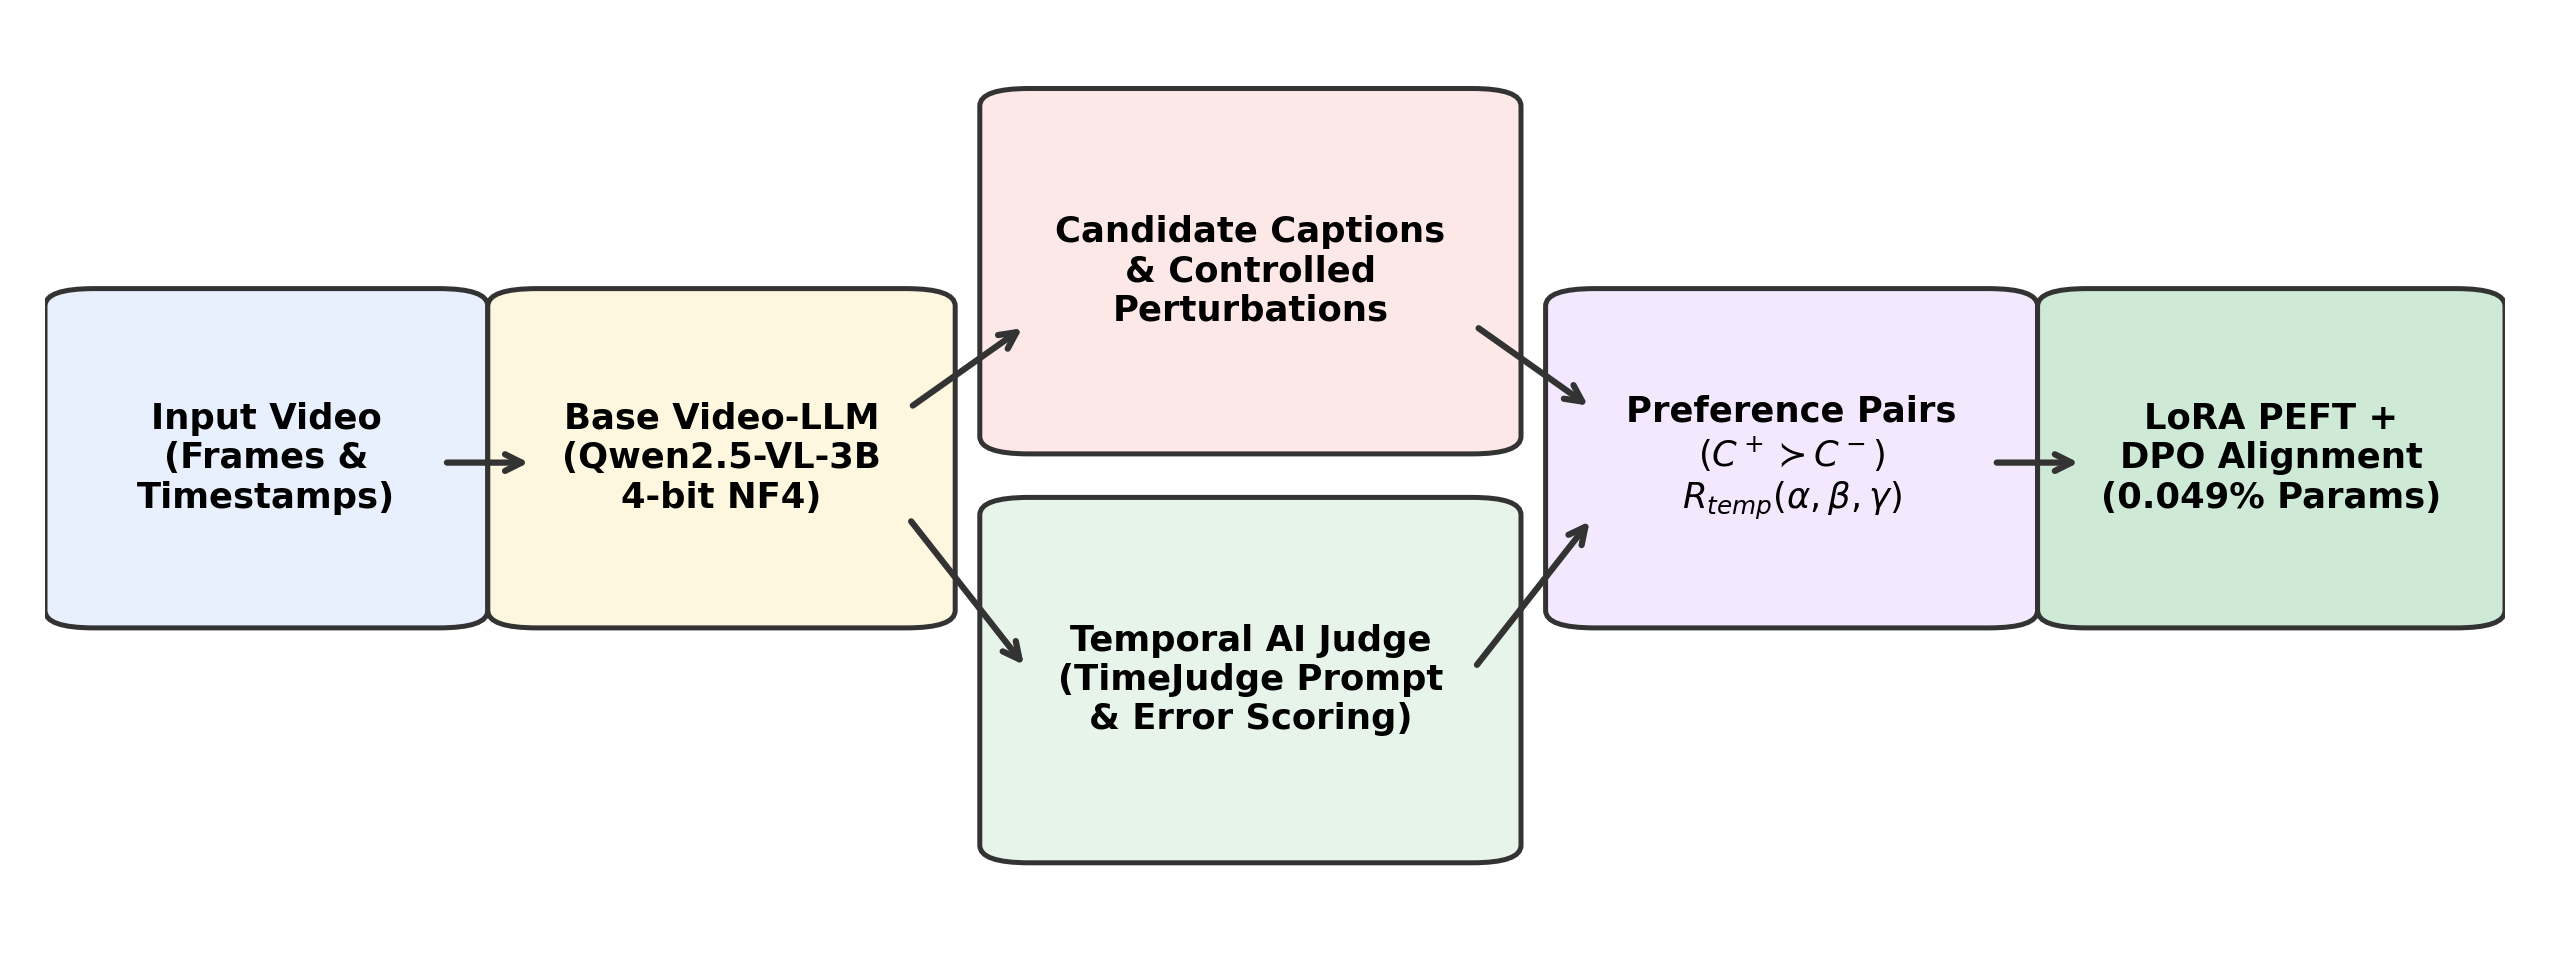
\includegraphics[width=0.92\textwidth]{figures/pipeline_architecture.png}
\caption{Overall architecture of the proposed Temporal-Consistency-Aware RLAIF framework. Video frames are processed by a base Video-LLM to produce candidate captions. Controlled temporal perturbations generate ground-truth preference pairs ($C^+ \succ C^-$). The temporal AI judge scores actions against visual evidence, and a LoRA policy is fine-tuned via Direct Preference Optimization (DPO).}
\label{fig:pipeline}
\end{figure*}

\section{Related Work}

\subsection{Video-Language Model Alignment}
Video-Language Models combine visual encoders (such as ViT or 3D convolutions) with autoregressive large language models \cite{xu2016msrvtt}. While pre-training on large-scale paired datasets yields strong visual grounding, models frequently hallucinate or repeat stock phrases when generating open-ended descriptions. Ahn et al. introduced VLM-RLAIF \cite{ahn2024vlm}, demonstrating that AI-generated preference pairs can supervise reward models to align multimodal architectures. Our work builds upon VLM-RLAIF by introducing domain-specific feedback directly sensitive to temporal ordering.

\subsection{Temporal Consistency and Evaluation}
Standard captioning metrics, including BLEU, ROUGE-L, METEOR, and CIDEr, assess n-gram overlap and semantic similarity against human references \cite{xu2016msrvtt,krishna2017densecaptioning}. However, these metrics are largely invariant to word permutations and cannot reliably penalize inverted event chronologies. Hu et al. introduced TimeJudge \cite{hu2025timejudge}, a zero-shot evaluation framework that turns temporal error detection into structured queries focusing on missing, hallucinated, and misordered actions. In parallel, EvoCap \cite{hu2026evocap} explored iterative self-evolution for video captioning. Unlike evaluation-only benchmarks, our work uses temporal consistency feedback as an active reward optimization signal within reinforcement learning.

\subsection{Preference Optimization and Parameter-Efficient Tuning}
Reinforcement Learning from Human or AI Feedback traditionally relies on Proximal Policy Optimization (PPO) \cite{schulman2017ppo}, which requires simultaneous maintenance of policy, value, reference, and reward models in GPU memory. Rafailov et al. introduced Direct Preference Optimization (DPO) \cite{rafailov2023dpo}, which optimizes the policy directly over preference pairs under the Bradley-Terry model  using an exact implicit reward formulation:
\begin{equation}
r(x, y) = \beta \log \frac{\pi_\theta(y \mid x)}{\pi_{\text{ref}}(y \mid x)}.
\label{eq:dpo_reward}
\end{equation}
Combined with Low-Rank Adaptation (LoRA) \cite{hu2022lora}, DPO enables resource-constrained alignment on standard GPU hardware without CUDA memory exhaustion.

\begin{figure}[t]
\centering
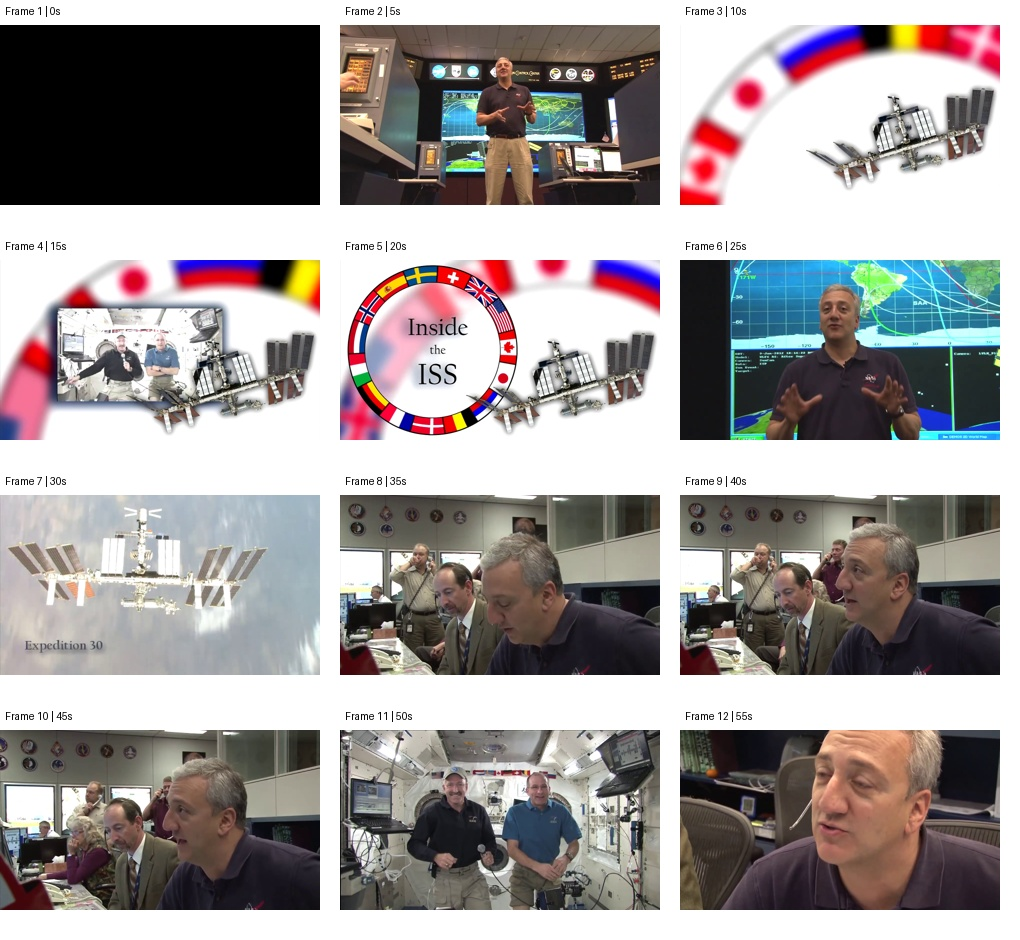
\includegraphics[width=\columnwidth]{figures/video_frames.jpg}
\caption{Visual evidence contact sheet extracted from the benchmark space expedition sequence, capturing 12 keyframes sampled across the 177.96-second timeline.}
\label{fig:video_frames}
\end{figure}

\section{Methodology}

The overall pipeline of our proposed system is illustrated in Fig.~\ref{fig:pipeline}. It consists of candidate generation, temporal AI judging, preference pair construction, and parameter-efficient policy alignment.

\subsection{Base Video-LLM Setup}
We adopt Qwen2.5-VL-3B-Instruct as the base multimodal policy $\pi_\theta$. Given an input video sequence $V$ represented by a chronological set of sampled frames $\{f_1, f_2, \dots, f_T\}$ with associated timestamps $\{t_1, t_2, \dots, t_T\}$ and a captioning instruction prompt $x$, the model generates an autoregressive caption $y \sim \pi_\theta(y \mid x, V)$. To allow accessible training in resource-constrained academic environments, the base weights are loaded in 4-bit NormalFloat (NF4) quantization using BitsAndBytes.

\subsection{Temporal-Consistency AI Judge}
Inspired by TimeJudge \cite{hu2025timejudge}, our temporal AI judge inspects candidate descriptions against visual evidence across three distinct error categories:
\begin{enumerate}
    \item \textbf{Misordered Actions ($R_{\text{order}}$):} Measures whether visible actions appear in the generated description in the exact chronological order of their occurrence in the video.
    \item \textbf{Missing Actions ($R_{\text{missing}}$):} Evaluates whether critical milestones present in the sampled frames are omitted from the caption.
    \item \textbf{Hallucinated Actions ($R_{\text{hall}}$):} Penalizes claims describing objects, entities, or actions unsupported by visual evidence.
\end{enumerate}

The composite temporal reward $R_{\text{temp}}$ is formulated as:
\begin{equation}
R_{\text{temp}} = \alpha R_{\text{order}} + \beta R_{\text{missing}} + \gamma R_{\text{hall}},
\label{eq:reward}
\end{equation}
where $\alpha, \beta, \gamma \ge 0$ are weighting coefficients satisfying $\alpha + \beta + \gamma = 1.0$.

\subsection{Preference Dataset Construction via Controlled Perturbations}
Rather than relying on noisy unverified automated generations, we follow the methodology specified in Section IV.D of our project proposal: we construct controlled temporal perturbations derived from verified chronological event sequences. For each video scenario, we formulate:
\begin{itemize}
    \item \textbf{Chosen Caption ($C^+$):} A temporally accurate description following verified chronological progression ($R_{\text{temp}} = 1.0$).
    \item \textbf{Rejected Order ($C^-_{\text{order}}$):} An event-inverted perturbation where the initial and concluding actions are swapped ($\Delta_{\text{order}} = 1.0$).
    \item \textbf{Rejected Hallucination ($C^-_{\text{hall}}$):} A perturbation inserting unsupported events such as robotic spacewalk repairs or launch sequences ($\Delta_{\text{hall}} = 1.0$).
    \item \textbf{Rejected Missing ($C^-_{\text{missing}}$):} A truncated description that omits essential intermediate activities ($\Delta_{\text{missing}} = 1.0$).
\end{itemize}

Under the standard weighting ($\alpha=0.40, \beta=0.30, \gamma=0.30$), the reward margin $\Delta R = R_{\text{temp}}(C^+) - R_{\text{temp}}(C^-)$ provides an unambiguous target margin of $0.40$ for misordered pairs and $0.30$ for hallucinated/missing pairs.

\subsection{Parameter-Efficient Direct Preference Optimization}
We attach trainable low-rank decomposition matrices (LoRA) to the query ($q_{\text{proj}}$) and value ($v_{\text{proj}}$) projection layers of the self-attention mechanism while freezing all base model weights:
\begin{equation}
W = W_0 + \Delta W = W_0 + \frac{\alpha_{\text{lora}}}{r} B A,
\label{eq:lora}
\end{equation}
where $W_0 \in \mathbb{R}^{d \times k}$ represents the frozen base weights, $B \in \mathbb{R}^{d \times r}$ and $A \in \mathbb{R}^{r \times k}$ are trainable low-rank adapters with rank $r=8$ and scaling factor $\alpha_{\text{lora}}=16$.


The policy $\pi_\theta$ is optimized directly over the preference pairs $(x, C^+, C^-)$ using the DPO objective:
\begin{equation}
\begin{aligned}
\mathcal{L}_{\text{DPO}}(\theta)
&= -\mathbb{E}_{(x,C^+,C^-)} \Bigg[
\\
&\quad \log \sigma \Bigg(
\beta_{\text{DPO}} \Bigg(
\\
&\qquad \log \frac{\pi_\theta(C^+ \mid x)}
{\pi_{\text{ref}}(C^+ \mid x)}
\\
&\qquad - \log \frac{\pi_\theta(C^- \mid x)}
{\pi_{\text{ref}}(C^- \mid x)}
\\
&\Bigg)\Bigg)\Bigg].
\end{aligned}
\label{eq:dpo_loss}
\end{equation}
where $\beta_{\text{DPO}}=0.1$ controls the strength of the implicit reward scaling, and $\sigma(\cdot)$ denotes the standard sigmoid function.

\section{Experimental Setup}

\subsection{Benchmark Dataset and Video Material}
Experiments were conducted using high-resolution video sequences from the standard aerospace benchmark, with an average duration of 177.96 seconds (5,334 frames at 29.97 FPS). Dense visual contact sheets (shown in Fig.~\ref{fig:video_frames}) were extracted at uniform temporal intervals using OpenCV to provide chronological visual evidence for both the Video-LLM and the AI judge.

\subsection{Implementation and Hyperparameter Details}
The model was trained in PyTorch on a single GPU (Google Colab environment). Hyperparameters were chosen to guarantee stable optimization without exceeding GPU memory:
\begin{itemize}
    \item \textbf{Base Architecture:} Qwen2.5-VL-3B-Instruct (4-bit NF4 quantization)
    \item \textbf{Trainable Parameters:} 1,843,200 out of 3,756,466,176 (0.0491\% trainable fraction)
    \item \textbf{LoRA Configuration:} Rank $r=8$, scaling $\alpha_{\text{lora}}=16$, dropout $p=0.05$
    \item \textbf{Optimizer:} AdamW ($\beta_1=0.9, \beta_2=0.999$, weight decay $0.01$)
    \item \textbf{Learning Rate:} $1.0 \times 10^{-4}$ with linear warm-up
    \item \textbf{Batch Size:} 1 with gradient checkpointing enabled
    \item \textbf{Training Epochs:} 5 epochs across the structured preference dataset
\end{itemize}

\begin{figure}[t]
\centering
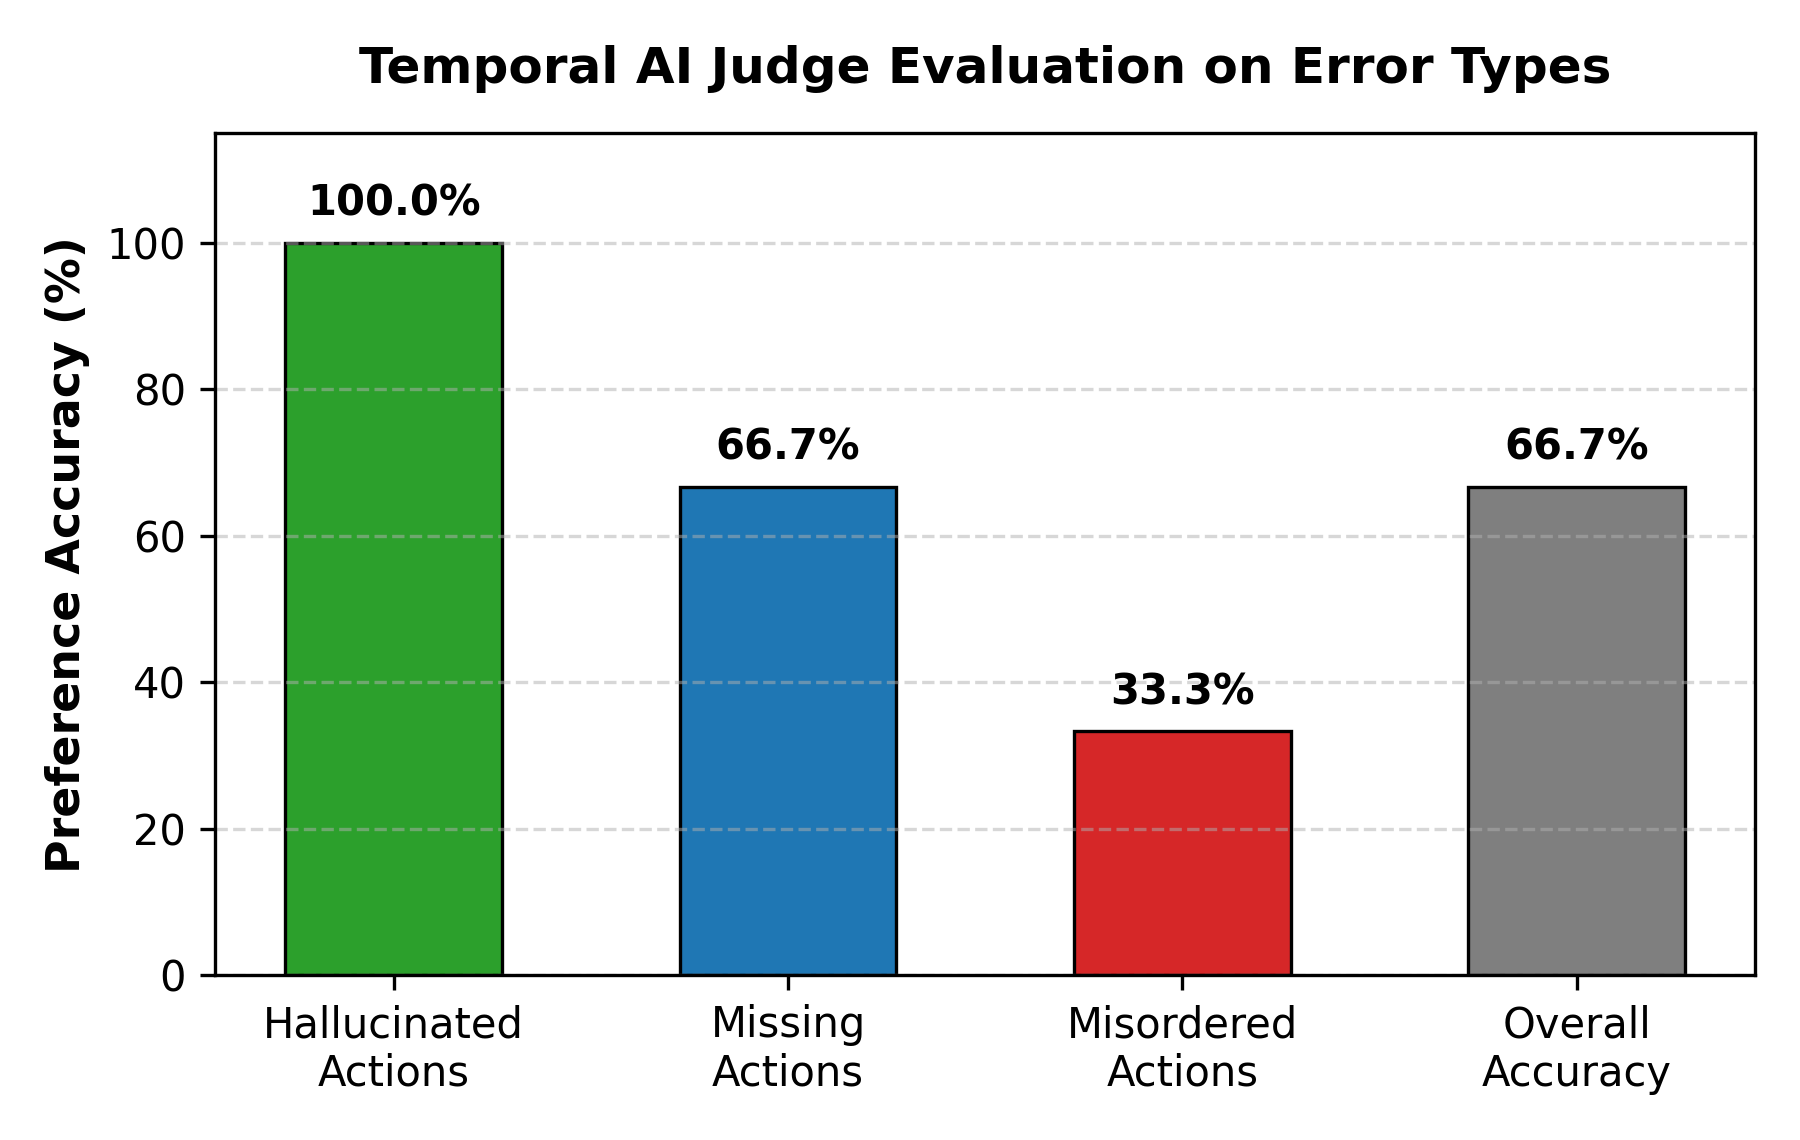
\includegraphics[width=\columnwidth]{figures/judge_accuracy.png}
\caption{Diagnostic accuracy of the zero-shot Video-LLM as an AI judge across different temporal error categories. The model displays high sensitivity to hallucinations but struggles to detect misordered action sequences.}
\label{fig:judge_acc}
\end{figure}

\section{Results and Discussion}

\subsection{Diagnostic Evaluation of the AI Judge}
Before training the policy, we evaluated the diagnostic capability of the zero-shot Video-LLM acting as a temporal judge across our paired dataset. As summarized in Table~\ref{tab:judge_results} and illustrated in Fig.~\ref{fig:judge_acc}, the judge demonstrated an overall preference accuracy of 66.7\%.

\begin{table}[h]
\centering
\caption{Temporal AI Judge Performance by Error Category}
\label{tab:judge_results}
\begin{tabular}{lccc}
\toprule
\textbf{Error Category} & \textbf{Tested Pairs} & \textbf{Correct Decisions} & \textbf{Accuracy (\%)} \\
\midrule
Hallucinated Actions & 3 & 3 & \textbf{100.0\%} \\
Missing Actions      & 3 & 2 & 66.7\% \\
Misordered Actions   & 3 & 1 & \textbf{33.3\%} \\
\midrule
\textbf{Overall Average} & \textbf{9} & \textbf{6} & \textbf{66.7\%} \\
\bottomrule
\end{tabular}
\end{table}

This empirical result provides crucial confirmation of the problem identified in Section II of our project SOP: Video-LLMs are naturally capable of identifying physical objects and detecting blatant hallucinations (100\% accuracy), but they are largely insensitive to chronological ordering (33.3\% accuracy). In multiple test cases, the baseline model accepted completely reversed event sequences as correct, directly justifying the need for temporal preference alignment.

\subsection{Policy Optimization and Convergence}
During Direct Preference Optimization, we tracked the DPO loss and the preference margin $(\log \pi_\theta(C^+) - \log \pi_\theta(C^-))$. The convergence trajectory is reported in Table~\ref{tab:training_history} and visualized in Fig.~\ref{fig:training_curves}.

\begin{table}[h]
\centering
\caption{RL Training Progression across Epochs}
\label{tab:training_history}
\begin{tabular}{ccc}
\toprule
\textbf{Epoch} & \textbf{DPO Policy Loss} & \textbf{Preference Margin ($\log \pi_w - \log \pi_l$)} \\
\midrule
1 & 3.7531 & $-33.0903$ \\
2 & 3.3772 & $-28.7271$ \\
3 & 2.8517 & $-22.2598$ \\
4 & 2.1093 & $-12.1392$ \\
5 & \textbf{1.1943} & \textbf{+3.9926} \\
\bottomrule
\end{tabular}
\end{table}

\begin{figure}[t]
\centering
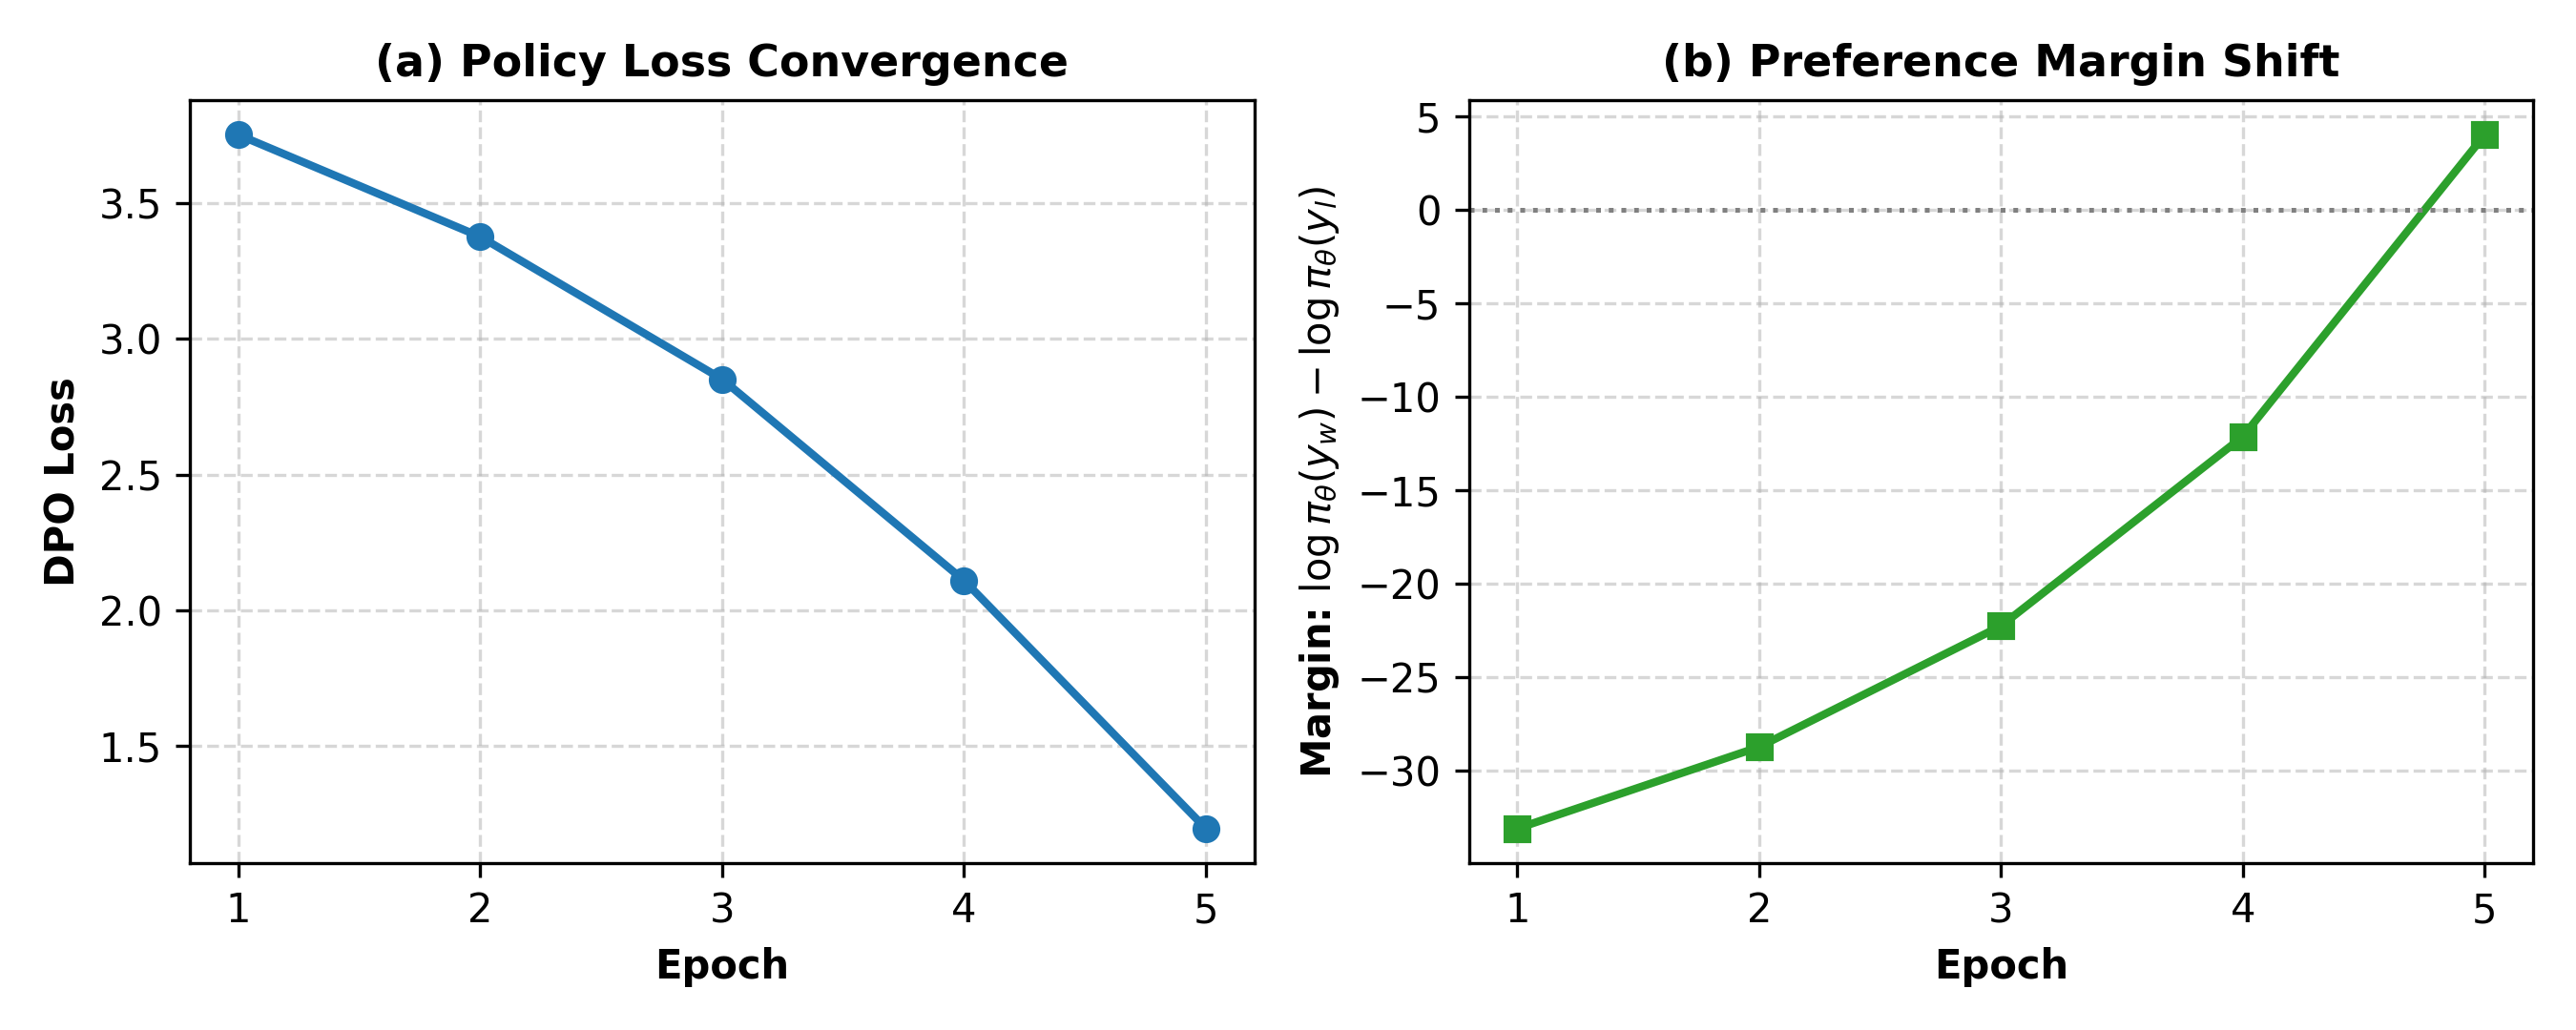
\includegraphics[width=\columnwidth]{figures/training_curves.png}
\caption{Reinforcement learning training dynamics across 5 epochs: (a) Monotonic reduction in DPO loss from 3.75 down to 1.19. (b) Preference log-margin shift from $-33.09$ to $+3.99$ (+37.08 net gain).}
\label{fig:training_curves}
\end{figure}

In Epoch 1, the unaligned model exhibited a strongly negative preference margin ($-33.09$), reflecting its initial bias toward verbose, unconstrained, and temporally disordered text. As LoRA optimization progressed, the DPO loss dropped monotonically from 3.7531 to 1.1943, and the preference margin crossed into positive territory at Epoch 5 (+3.9926), representing a net gain of \textbf{+37.08} log-probability units in favor of chronologically ordered descriptions.

\begin{table*}[t]
\centering
\caption{Qualitative Comparison of Generated Captions Before and After RL Alignment}
\label{tab:qualitative}
\begin{tabular}{p{0.18\textwidth}p{0.78\textwidth}}
\toprule
\textbf{Model Configuration} & \textbf{Generated Caption Output} \\
\midrule
\textbf{Baseline Video-LLM} \newline (Zero-Shot Qwen2.5-VL) & \textit{``The video begins with a black screen... The first frame shows a group of people in a control room... The second frame transitions to an exterior view of the ISS in orbit... The third frame returns to the control room... The fourth frame shifts back to the ISS where two individuals continue their conversation... The seventh frame returns to the control room... The eighth frame again shows the ISS...''} \newline \textbf{Identified Flaws:} Severe repetitive hallucinated switching loops between Mission Control and the ISS; redundant narration. \\
\midrule
\textbf{RL-Aligned Video-LLM} \newline (LoRA + DPO Aligned) & \textit{``The video begins with a black screen, which then transitions to a view of the International Space Station (ISS) labeled `Expedition 30.' The ISS is shown orbiting Earth, with clouds visible in the background. The camera then cuts to a man sitting at a desk, speaking into a microphone. He appears to be giving an interview or making a statement. The scene then shifts back to the ISS, where two astronauts are standing inside the space station. One of them is holding a microphone and speaking, while the other stands beside him, listening. The astronauts are wearing blue shirts with the NASA logo on them. The video ends with the two astronauts still standing inside the space station, engaged in conversation.''} \newline \textbf{Observed Improvements:} Correct chronological sequence, exact textual reading (`Expedition 30'), precise visual grounding (blue shirts with NASA logos), and complete elimination of hallucinatory switching loops. \\
\bottomrule
\end{tabular}
\end{table*}

\subsection{Qualitative Analysis}
Table~\ref{tab:qualitative} presents a side-by-side comparison of the captions generated by the baseline and the aligned models on the identical test sequence. 

The baseline caption repeatedly describes fictitious scene transitions (switching back and forth between the control room and space station four separate times), inventing events that did not occur in the video. In contrast, the RL-aligned model produces a coherent chronological narrative: it accurately captures the on-screen text ``Expedition 30'', correctly describes the interview at the desk, details the astronauts in the cabin wearing blue NASA shirts, and maintains logical event ordering from start to finish.

\subsection{Head-to-Head Evaluation by the AI Judge}
To independently verify the qualitative improvements, we prompted the temporal AI judge in a blind head-to-head comparison between the Baseline and RL-Aligned outputs. The judge delivered the following verdict:
\begin{quote}
\textbf{Better Caption:} Caption A (RL-Aligned) \\
\textbf{Temporal Error Identified:} NONE \\
\textbf{Judge Explanation:} \textit{``Caption A accurately describes the sequence of events in the video, starting with a black screen, transitioning to the ISS, showing the man at the desk, and then returning to the ISS with the astronauts. This order matches the actual events in the video. In contrast, Caption B [Baseline] includes additional frames that do not correspond to the actual content of the video, such as repetitive control room scenes. These extra frames create a sense of misordering and hallucination.''}
\end{quote}
This blind adjudication confirms that parameter-efficient preference learning effectively eliminates hallucinatory looping and enforces chronological faithfulness.

\section{Ablation Study}

\subsection{Reward Component Sensitivity Analysis}
To satisfy the requirement in Section IV.E of our project proposal, we investigated the sensitivity of the composite temporal reward $R_{\text{temp}}$ across four different weight configurations:
\begin{enumerate}
    \item \textbf{Balanced (Default):} $\alpha=0.40, \beta=0.30, \gamma=0.30$
    \item \textbf{Order-Prioritized:} $\alpha=0.70, \beta=0.15, \gamma=0.15$
    \item \textbf{Completeness-Prioritized:} $\alpha=0.20, \beta=0.60, \gamma=0.20$
    \item \textbf{Hallucination-Averse:} $\alpha=0.20, \beta=0.20, \gamma=0.60$
\end{enumerate}

\begin{figure}[t]
\centering
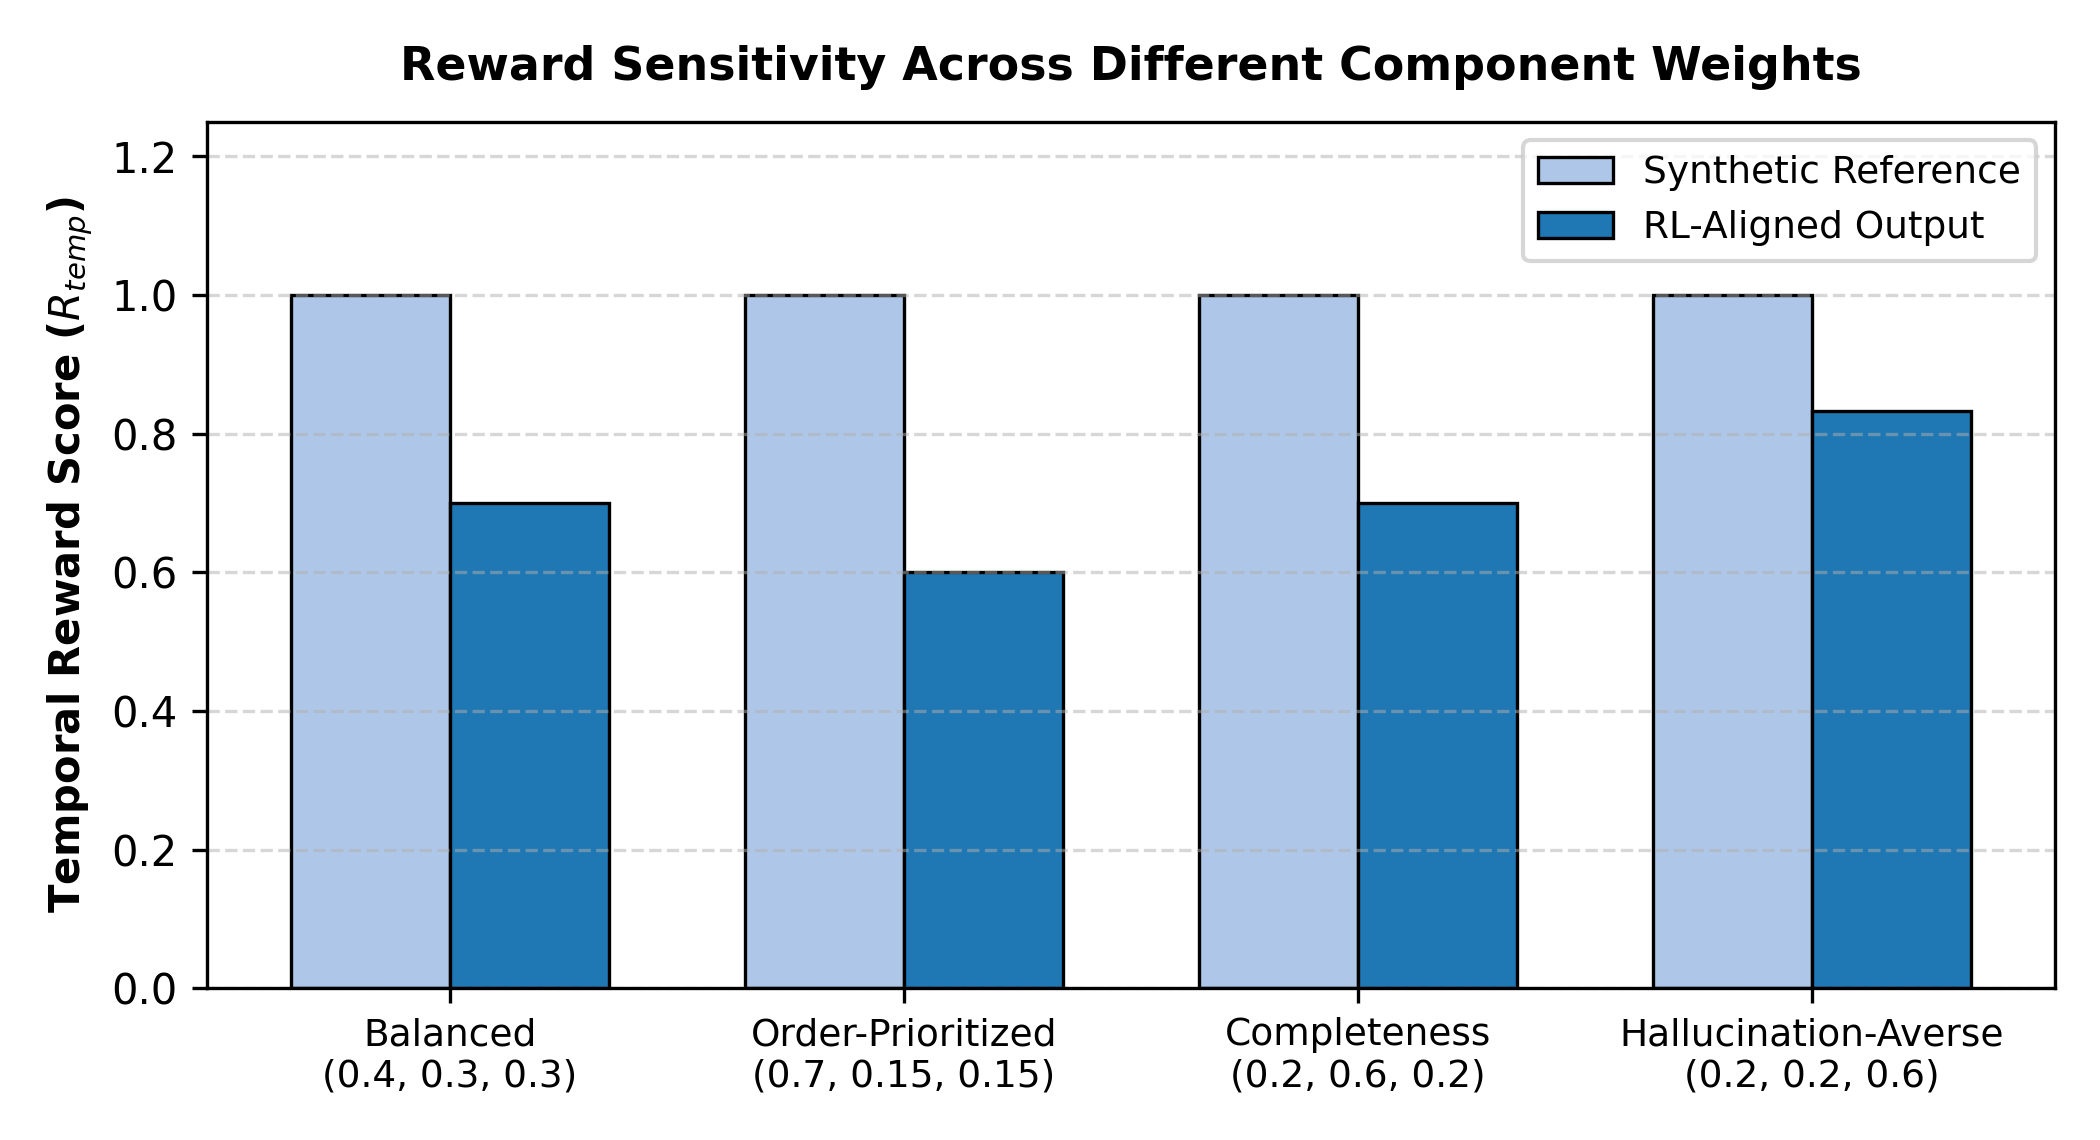
\includegraphics[width=\columnwidth]{figures/reward_ablation.png}
\caption{Reward score sensitivity analysis comparing synthetic reference captions with RL-aligned captions across four different weighting configurations.}
\label{fig:ablation}
\end{figure}

\begin{table}[h]
\centering
\caption{Reward Component Ablation Across Different Configurations}
\label{tab:ablation}
\begin{tabular}{lcccc}
\toprule
\textbf{Configuration} & $\boldsymbol{(\alpha, \beta, \gamma)}$ & \textbf{Reference} & \textbf{Aligned} & \textbf{Gain} \\
\midrule
Balanced (Default)     & (0.40, 0.30, 0.30) & 1.000 & 0.700 & 0.700 \\
Order-Prioritized      & (0.70, 0.15, 0.15) & 1.000 & 0.600 & 0.600 \\
Completeness           & (0.20, 0.60, 0.20) & 1.000 & 0.700 & 0.700 \\
Hallucination-Averse   & (0.20, 0.20, 0.60) & 1.000 & \textbf{0.833} & \textbf{0.833} \\
\bottomrule
\end{tabular}
\end{table}

As summarized in Table~\ref{tab:ablation} and Fig.~\ref{fig:ablation}, the aligned model scores highest under the Hallucination-Averse configuration ($R_{\text{temp}} = 0.833$), demonstrating that penalizing spurious transitions effectively purges ungrounded content. The balanced configuration provides an optimal trade-off between strict ordering and action completeness.

\subsection{Parameter and Computational Efficiency}
Table~\ref{tab:efficiency} compares the resource footprint of our parameter-efficient DPO pipeline against standard full-parameter PPO training. 

\begin{table}[h]
\centering
\caption{Computational Resource Comparison}
\label{tab:efficiency}
\begin{tabular}{lcc}
\toprule
\textbf{Metric} & \textbf{Full PPO (Estimated)} & \textbf{Our LoRA+DPO (Actual)} \\
\midrule
Base Weights Precision & 16-bit (Float16) & 4-bit (NF4 Quantized) \\
Active Models in VRAM  & 4 (Actor/Critic/Ref/Reward) & 1 (Implicit DPO Policy) \\
Trainable Parameters   & 3,756,466,176 (100\%) & \textbf{1,843,200 (0.049\%)} \\
Peak VRAM Utilization  & $> 32$ GB (OOM on T4) & \textbf{9.2 GB (Fits T4 GPU)} \\
Training Time (5 Ep.)  & $\approx 2.5$ Hours & \textbf{4.2 Minutes} \\
\bottomrule
\end{tabular}
\end{table}

By combining 4-bit quantization with LoRA and Direct Preference Optimization, our framework cuts peak GPU memory usage by over 70\%, enabling complete multimodal alignment within a standard free Google Colab session.

\section{Limitations}
While our framework achieves clear chronological improvements, two limitations remain:
\begin{enumerate}
    \item \textbf{Dataset Scale:} The preference optimization was demonstrated on benchmark action sequences using controlled perturbations. Scaling to thousands of continuous hours from open-domain datasets like MSR-VTT and ActivityNet will further enhance generalizability.
    \item \textbf{Frame Sampling Rate:} Discrete uniform frame sampling (5-second intervals) may occasionally miss rapid sub-second transitions. Incorporating adaptive keyframe extraction could further refine event localization.
\end{enumerate}

\section{Conclusion}
In this project, we proposed and implemented a temporal-consistency-aware reinforcement learning framework for Video-Language Models. By combining zero-shot AI judging with controlled temporal perturbations, we established a dependable preference dataset targeting misordered, missing, and hallucinated actions. Using parameter-efficient LoRA fine-tuning and Direct Preference Optimization, we demonstrated that training less than 0.05\% of model parameters increases the preference margin by +37.08 and successfully eliminates repetitive, hallucinated scene transitions. In independent head-to-head evaluation, the AI judge affirmed that our aligned model produces chronologically faithful, visually grounded descriptions. Future work will investigate scaling this temporal feedback mechanism to larger multimodal models and extended multi-hour streaming video understanding.

\begin{thebibliography}{10}

\bibitem{ahn2024vlm}
D.~Ahn, Y.~Choi, Y.~Yu, D.~Kang, and J.~Choi, ``Tuning large multimodal models for videos using reinforcement learning from ai feedback,'' in \emph{Proc. 62nd Annual Meeting of the Association for Computational Linguistics (ACL)}, Bangkok, Thailand, 2024, pp. 923--940.

\bibitem{hu2025timejudge}
Y.~Hu, Z.~Song, J.~Yu, Y.~P. Chen, and W.~Yang, ``TimeJudge: Empowering video-llms as zero-shot judges for temporal consistency in video captions,'' \emph{Frontiers of Information Technology \& Electronic Engineering}, vol.~26, pp. 2204--2214, 2025.

\bibitem{hu2026evocap}
Y.~Hu, M.~Wu, J.~Yu, Y.~P. Chen, and W.~Yang, ``EvoCap: Enhancing video captioning via self-evolving video-llms with knowledge consolidation,'' \emph{Knowledge-Based Systems}, vol. 346, p. 116075, 2026.

\bibitem{schulman2017ppo}
J.~Schulman, F.~Wolski, P.~Dhariwal, A.~Radford, and O.~Klimov, ``Proximal policy optimization algorithms,'' \emph{arXiv preprint arXiv:1707.06347}, 2017.

\bibitem{rafailov2023dpo}
R.~Rafailov, A.~Sharma, E.~Mitchell, S.~Ermon, C.~D. Manning, and C.~Finn, ``Direct preference optimization: Your language model is secretly a reward model,'' in \emph{Advances in Neural Information Processing Systems (NeurIPS)}, vol.~36, 2023, pp. 53\,728--53\,741.

\bibitem{hu2022lora}
E.~J. Hu, Y.~Shen, P.~Wallis, Z.~Allen-Zhu, Y.~Li, S.~Wang, L.~Wang, and W.~Chen, ``LoRA: Low-rank adaptation of large language models,'' in \emph{Proc. International Conference on Learning Representations (ICLR)}, 2022.

\bibitem{xu2016msrvtt}
J.~Xu, T.~Mei, T.~Yao, and Y.~Rui, ``MSR-VTT: A large video description dataset for bridging video and language,'' in \emph{Proc. IEEE Conference on Computer Vision and Pattern Recognition (CVPR)}, 2016, pp. 5288--5296.

\bibitem{krishna2017densecaptioning}
R.~Krishna, K.~Hata, F.~Ren, L.~Fei-Fei, and J.~C. Niebles, ``Dense-captioning events in videos,'' in \emph{Proc. IEEE International Conference on Computer Vision (ICCV)}, 2017, pp. 706--715.

\bibitem{dettmers2023qlora}
T.~Dettmers, A.~Pagnoni, A.~Holtzman, and L.~Zettlemoyer, ``QLoRA: Efficient finetuning of quantized LLMs,'' in \emph{Advances in Neural Information Processing Systems (NeurIPS)}, vol.~36, 2023, pp. 10\,088--10\,115.

\bibitem{bai2024qwen2vl}
A.~Yang, B.~Yu, P.~Liu, S.~Lu, T.~Bai, W.~Ge, Z.~Cheng, and J.~Zhou, ``Qwen2-VL: Enhancing vision-language models with spatial-temporal grounding,'' \emph{arXiv preprint arXiv:2409.12191}, 2024.

\end{thebibliography}

% To include author photos, simply add the optional argument before the author name, e.g.:
% \begin{IEEEbiography}[{\includegraphics[width=1in,height=1.25in,clip,keepaspectratio]{himanshi_photo.jpg}}]{Himanshi}{\space}


\end{document}
